
\RequirePackage{silence}
\documentclass[10pt, compress,british,xcolor={svgnames,dvipsnames,x11names},trans]{beamer}

\usepackage{babel}
\usepackage{csquotes}
\usepackage{comment}
\usepackage{tikzsymbols}


% OP - Ondrej Platek inline 
\definecolor{purple}{RGB}{200,0,200}
\def\OP#1{{\color{purple}OP: \it #1}}
\def\OPdel#1{\bgroup\markoverwith{\textcolor{purple}{\rule[0.5ex]{2pt}{1pt}}}\ULon{#1}}

%%% mtheme customisations
\usetheme[progressbar=frametitle,block=fill]{m}
\setmonofont[Scale=0.92]{Fira Mono}
\AtBeginSubsection{
\metroset{color/background=dark}
\frame[plain,c]{
  \begin{center}
  \begin{minipage}{25em}
    \usebeamercolor[fg]{section title}
    \usebeamerfont{section title}
    \insertsubsection\\[-1ex]
    \usebeamertemplate*{progress bar in section page}
  \end{minipage}
  \end{center}
}
\metroset{color/background=light}
}
%%%%% end mtheme

\setbeamertemplate{frametitle continuation}[from second]
\setbeamertemplate{bibliography item}[book]

\usepackage{xeCJK}
%\setCJKsansfont[BoldFont=Kozuka Gothic Pro]{Kozuka Gothic Pro L}
\setCJKsansfont{IPAGothic}
% \newCJKfontfamily{\xiheifont}[BoldFont=STHeiti]{STXihei}
\newCJKfontfamily{\xiheifont}{WenQuanYi Micro Hei}

\usetikzlibrary{arrows}
\usetikzlibrary{chains}
\usepackage{tikz-qtree}
\usepackage{multicol}


\usepackage{expex}
%\lingset{glhangindent=2em,glspace=1em,aboveexskip=0pt,belowexskip=0pt,aboveglftskip=-3pt,extraglskip=3pt} %v0.1
%\lingset{exskip=0pt,interpartskip=-3pt,belowpreambleskip=-3pt,belowglpreambleskip=-3pt,aboveglftskip=-3pt,extraglskip=3pt,glhangstyle=none}
\usepackage{relsize}
\usepackage{booktabs,tabularx}
%\usepackage{textcomp}
\usepackage{listings}
\lstset{basicstyle=\ttfamily,breaklines=true,breakatwhitespace=true,
keywordstyle={\color{NavyBlue}\bfseries}, showstringspaces=false,
commentstyle={\color{PaleVioletRed4}},
emphstyle={\color{OliveGreen}\bfseries}
}

\usepackage{algorithmic}
\renewcommand{\algorithmiccomment}[1]{\alert{/* #1 */}}

\usetikzlibrary{shapes.multipart}
\usetikzlibrary{positioning}
\usetikzlibrary{arrows.meta}

\makeatletter
\pgfarrowsdeclare{crow's foot}{crow's foot}
{
  \pgfarrowsleftextend{+-.5\pgflinewidth}%
  \pgfarrowsrightextend{+.5\pgflinewidth}%
}
{
  \pgfutil@tempdima=0.5pt%
  \advance\pgfutil@tempdima by.25\pgflinewidth%
  \pgfsetdash{}{+0pt}%
  \pgfsetmiterjoin%
  \pgfpathmoveto{\pgfqpoint{0pt}{-6\pgfutil@tempdima}}%
  \pgfpathlineto{\pgfqpoint{-6\pgfutil@tempdima}{0pt}}%
  \pgfpathlineto{\pgfqpoint{0pt}{6\pgfutil@tempdima}}%
  \pgfusepathqstroke%
}

\usepackage[os=win]{menukeys}


\title{RNNs for Dialogue State Tracking}


\author{Ondřej Plátek, Petr Bělohlávek, Vojtěch Hudeček \& Filip Jurčíček \\ \footnotesize{\texttt{vojta.hudecek@gmail.com,oplatek@ufal.mff.cuni.cz}}}
\institute{
Institute of Formal and Applied Linguistics\\
Faculty of Mathematics and Physics\\
Charles university in Prague
}

\begin{document}

\maketitle


%!TEX root = Intro-NLP-seminar.tex
\section{Introduction}

\begin{frame}
\frametitle{sample dialogue}
\begin{itemize}
\item[] 
\begin{itemize}
\item[] (\OP{cuisine->food}: ?, area: ?, price: ?)
\end{itemize}
\item[] System: \textit{What type of restaurant are you looking for?}
\begin{itemize}
\item[] \texttt{request(\OP{!cuisine!})}
\end{itemize}
\item[] User: \textit{I am looking for a japanese restaurant in the city center.}
\begin{itemize}
\item[] \texttt{inform(\OP{!cuisine!}:japanese, area:center)}
\end{itemize}
\item[] System: \textit{What price range do you prefer?}
\begin{itemize}
\item[] \texttt{request(price)}
\end{itemize}
\item[] User: \textit{I want something cheap.}
\begin{itemize}
\item[] \texttt{inform(price:cheap)}
\end{itemize}
\end{itemize}
\end{frame}

\begin{frame}
\frametitle{sample dialogue}
\begin{itemize}
\item[] 
\begin{itemize}
\item[] (cuisine: ?, area: ?, price: ?)
\end{itemize}
\item[] System: \textit{What type of restaurant are you looking for?}
\item[] User: \textit{I am looking for a japanese restaurant in the city center.}
\begin{itemize}
\item[] (\textcolor{red}{cuisine: japanese}, \textcolor{red}{area: center}, price: ?)
\end{itemize}
\item[] System: \textit{What price range do you prefer?}
\item[] User: \textit{I want something cheap.}
\begin{itemize}
\item[] (cuisine: japanese, area: center, \textcolor{red}{price: cheap})
\end{itemize}
\end{itemize}
\end{frame}

\begin{frame}
\frametitle{Why track a dialogue}
\begin{itemize}[<+->]
\item Dialogue agent tracks the progress and decides what action to take.
\begin{itemize}
\item \OP{?Essential information?}
\end{itemize}
\item Need to to represent the state \OP{?somehow?}
\item Track \OP{?obtained?} information (history)
\item \alert{What does the user probably want?} \OP{nerozumim}
\end{itemize}
\end{frame}

\begin{frame}
\frametitle{What is the Dialogue state}

\begin{itemize}[<+->]
\item Triple \texttt{(method, slot, value)}
\item State space of possible situations
\begin{itemize}
\item Each situation described e.g. by Dialog Act Item
\item Probability distribution over situations
\item \OP{Tracking just slots and values}
\end{itemize}
\item Example using Dialog Act Items:
	\begin{itemize}
	\item (\textcolor{red}{cuisine}: \textcolor{blue}{japanese}, \textcolor{red}{area}: \textcolor{blue}{center}, \textcolor{red}{price}: \textcolor{blue}{moderate})
	\end{itemize}
\end{itemize}
\end{frame}

%\begin{frame}
%\frametitle{Possible approaches\cite{zilka2013}}
%\begin{itemize}
%\item \textbf{Discriminative belief update}
%\begin{itemize}
%\item Belief state is a product of marginal probabilities of all pairs \textit{slot:value}
%\end{itemize}
%\item \textbf{Belief update with generative model}
%\begin{itemize}
%\item Distribution factorized into transition and observation model
%\item Bayesian network of possible values
%\end{itemize}
%\item Both can accumulate information 
%\item Discriminative model outperforms the generative one, however it is quite naive.
%\end{itemize}
%\end{frame}

\begin{frame}
\frametitle{DSTC2 Dataset\cite{Henderson2014a}}
\begin{itemize}
\item Challenge organized by University of Cambridge, dataset publicly available.
\item Each dialogue composed of \textit{turns} - pair of user and system utterances.
\item Annotated dialogues - gold DAI after each turn.
\end{itemize}

\end{frame}

\begin{frame}
\frametitle{DSTC2 Dataset}
\begin{itemize}
\item Train set contains 1612, development 506 and test 1117 dialogues
\item Dialogues were obtained by user-computer interaction
\item Mix of Dialogue Managers \OP{?Systems?} and ASR engines was used.
\begin{itemize}
\item Different setting used for each set \alert{$\rightarrow$ increased difficulty}
\item Reshuffled data significantly easier
\end{itemize}
\end{itemize}
\end{frame}

\section{Our model}
\begin{frame}
\frametitle{RNN Encoder-decoder}
\begin{columns}
\begin{column}{0.65\textwidth}
\begin{itemize}
\item Recurrent neural network composed of sequentially ordered cells
\item Maintains (encodes) hidden state and emits observation after each turn
\item Improved with LSTM cells
\item Suitable for DST task - history is taken into account
\end{itemize}
\end{column}
\begin{column}{0.35\textwidth}
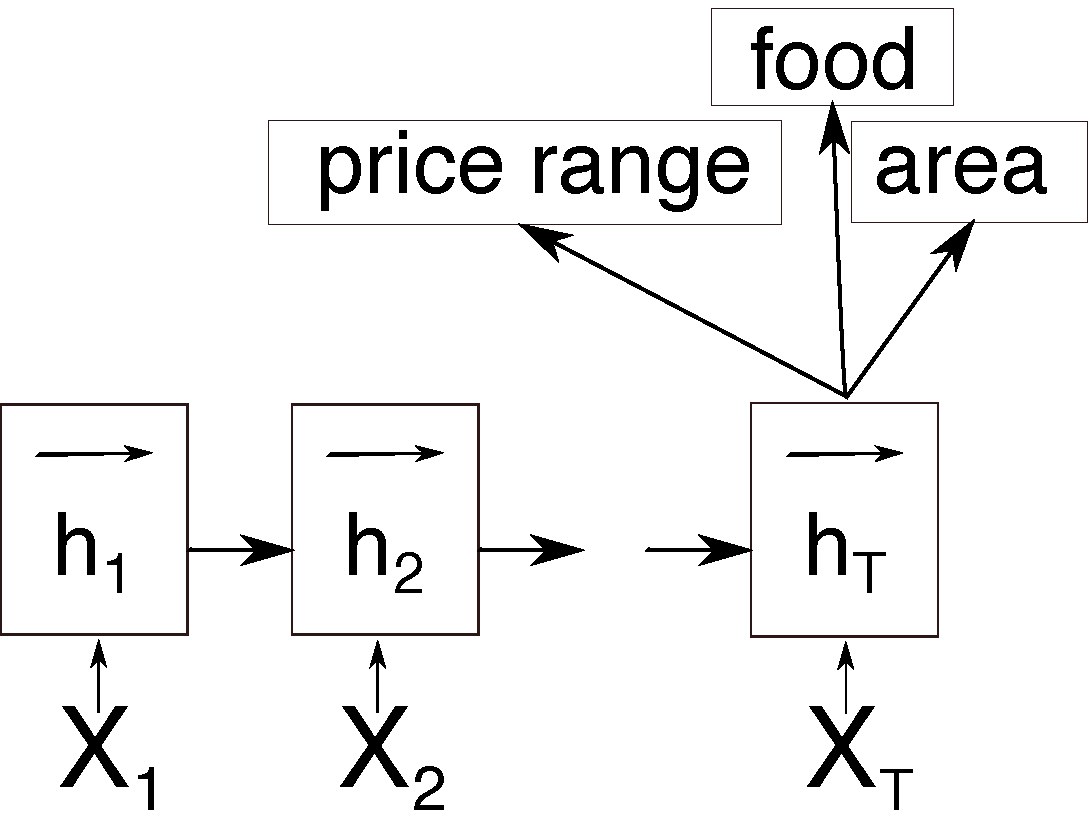
\includegraphics[width=0.90\textwidth]{encoder.pdf}
\end{column}
\end{columns}
\end{frame}

\begin{frame}
\frametitle{Model details}
\begin{itemize}
\item TensorFlow framework - good performance and desired functionality, e.g. GPU computation, \texttt{seq2seq}
\item Supervised learning
\item Predicting labels jointly or independently
\begin{itemize}
\item joint model suffers from data sparsity\
\end{itemize}
\end{itemize}
\end{frame}

\begin{frame}
\frametitle{Model details}
\begin{itemize}
\item INPUT FEATURES
\begin{itemize}
\item one-hot encoding (Bag of Words)
\item vector embeddings of words
\item indicator, whether the word belong to particular domain 
\end{itemize}
\item We do not predict the method - trivial
\end{itemize}
\end{frame}

\begin{frame}
\frametitle{Training and Evaluation}
\begin{itemize}
\item During training, each turn is predicted based on whole dialogue history
\item Data separated into buckets of similar lengths 
\item \textbf{Accuracy} metric was used, i.e. fraction of turns, where the most probable hypotheses was correct
\item \textbf{schedule 2} includes only turns, where some information is taken from the user
\end{itemize}
\end{frame}
\section{Results}
\begin{frame}
\frametitle{Results}
\begin{itemize}
\item Independent model achieved better results - 0.73
\item Comparable to models that use whole list of ASR hypothesis
\item Much better performance of both models on the reshuffled data

\end{itemize}
\end{frame}
\begin{frame}
\frametitle{Conclusion}
\begin{itemize}
\item We successfully used the encoder-decoder model for DST task and achieved promising results
\item We verified that DSTC2 difficulty stems from the use of different settings
\end{itemize}
\end{frame}

\begin{frame}
\frametitle{Future work}
\begin{itemize}
\item The model could be further improved by employment of other features
\item World-level annotated dataset would help to evaluate the incremental models
\end{itemize}
\end{frame}

\plain{The End\\Thank you!}

\appendix
\begin{frame}[allowframebreaks]
        \frametitle{References}
        \bibliographystyle{plain}
        \bibliography{refs.bib}
\end{frame}

\end{document}